\documentclass[11pt]{article}
\usepackage[utf8]{inputenc}
\usepackage{graphicx}
\usepackage{subfig}
\usepackage{enumerate}
\usepackage{fourier}
\usepackage[T1]{fontenc}
% \usepackage[letter,width=150mm, top=30mm, bottom=30mm]{geometry}
\usepackage[font={footnotesize}]{caption}
\usepackage[labelfont=bf]{caption}
\usepackage[english]{babel}
\usepackage{amsmath}
\usepackage{fontspec}

\setlength{\parskip}{1em}
\graphicspath{{../figs/}}

\title{Practice Session 02: Uncertainties in Stress Inversion}
\author{Prithvi Thakur}
\date{Feb 13, 2019}

\begin{document}

\maketitle

% Problem 1
\section*{Principal stresses in the Sumatra-Andaman region}
We divide the Sumatra-Andaman oblique subduction zone into two regions  based on the strike of the subduztion zone. Ideally, we would separate the region based on the change in strike as well as dip to account for the different parts of the tectonic plates.

Here, we will focus on the Projection 1 in the Fig. 1. The total number of data sets in our region defined by projection 1 is 496. It is predominantly a strike slip setting. We will look at smaller subsets of the data and see how the uncertainty due to bootstrapping varies.

\begin{figure}[!htb]
    \centering
    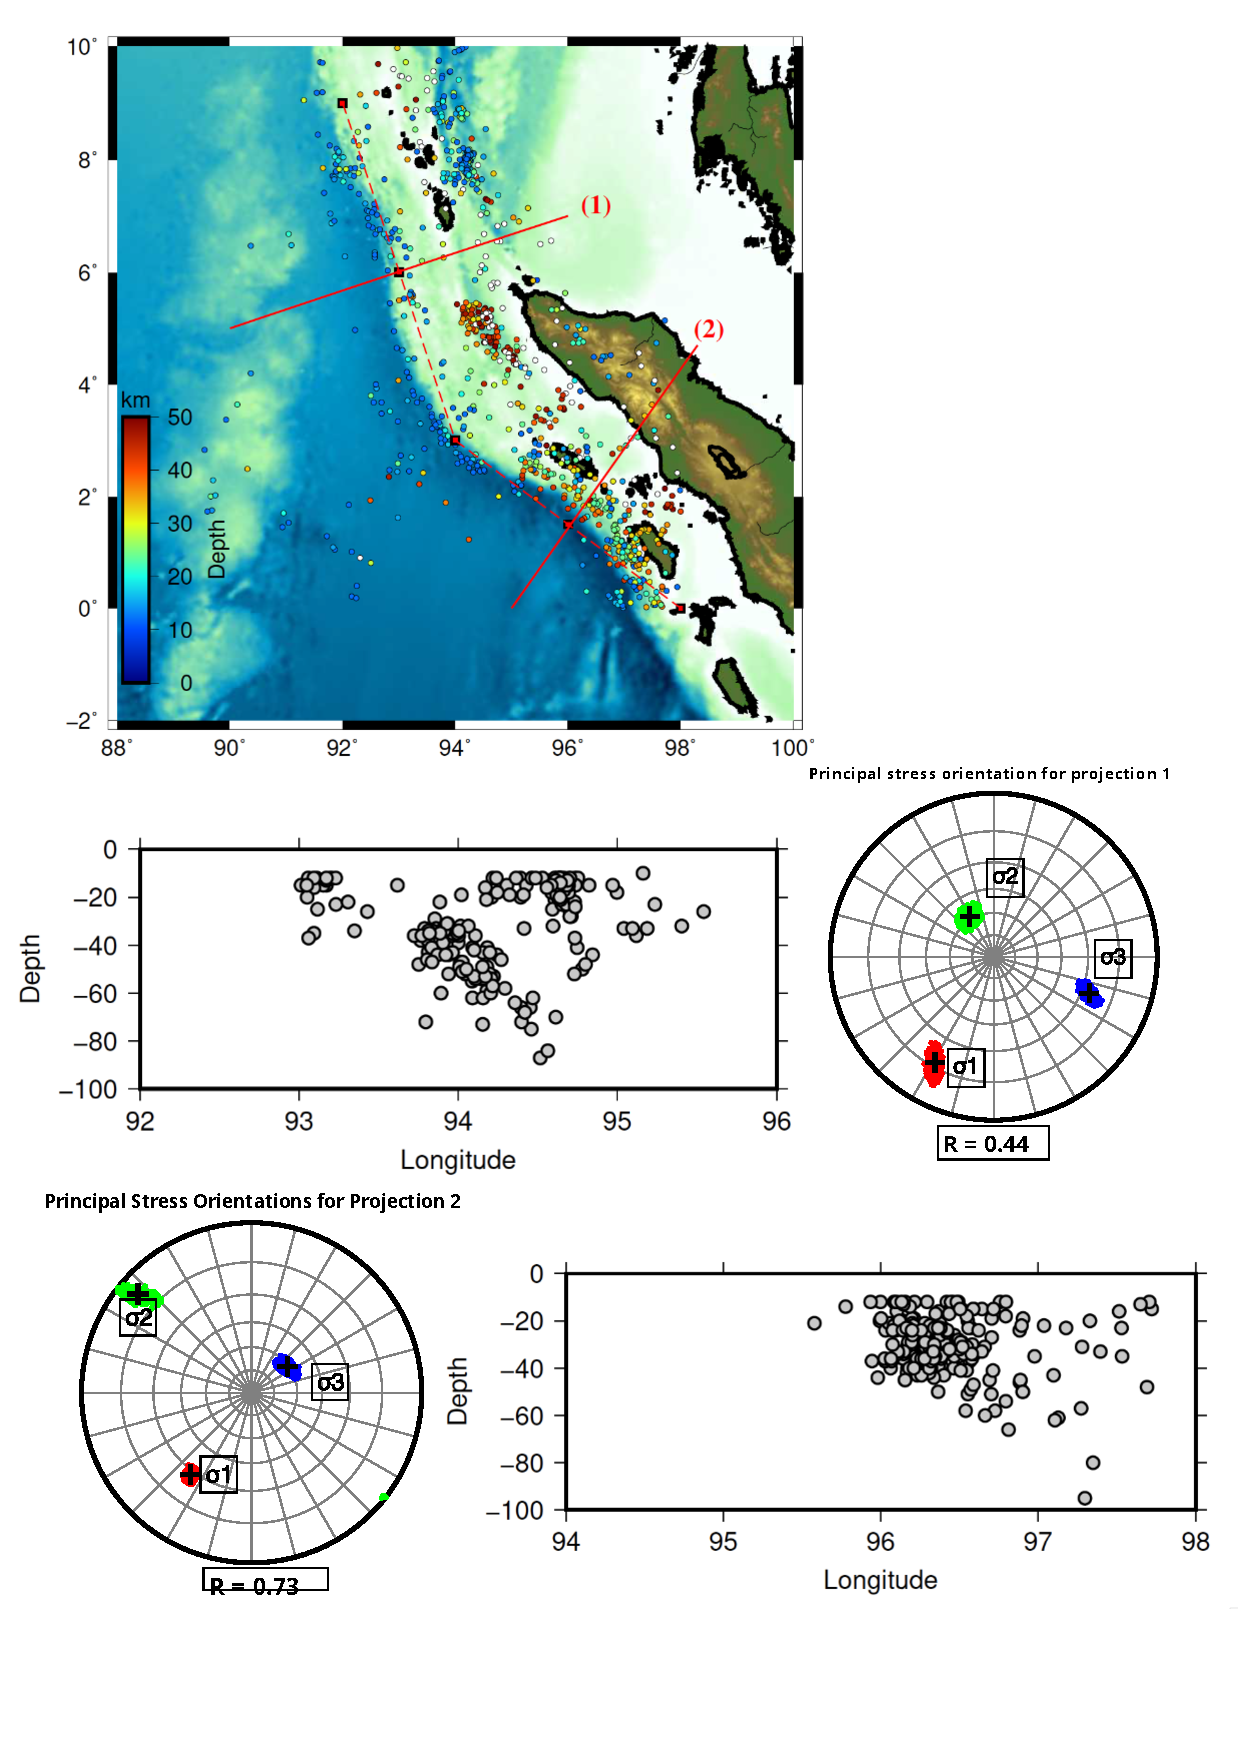
\includegraphics[scale=0.7]{fig1.pdf}
\end{figure}

\section*{Uncertainty due to change in the number of earthquakes/data points}
Our data set of 496 earthquakes includes all the earthquakes recorded from 1970-present. We divide the 496 earthquakes into smaller data sets systematically, ensuring that each fault and nodal plane are within the same data set. The stress inversion for different data sizes are shown below: 

\begin{figure}[!htb]
    \centering
    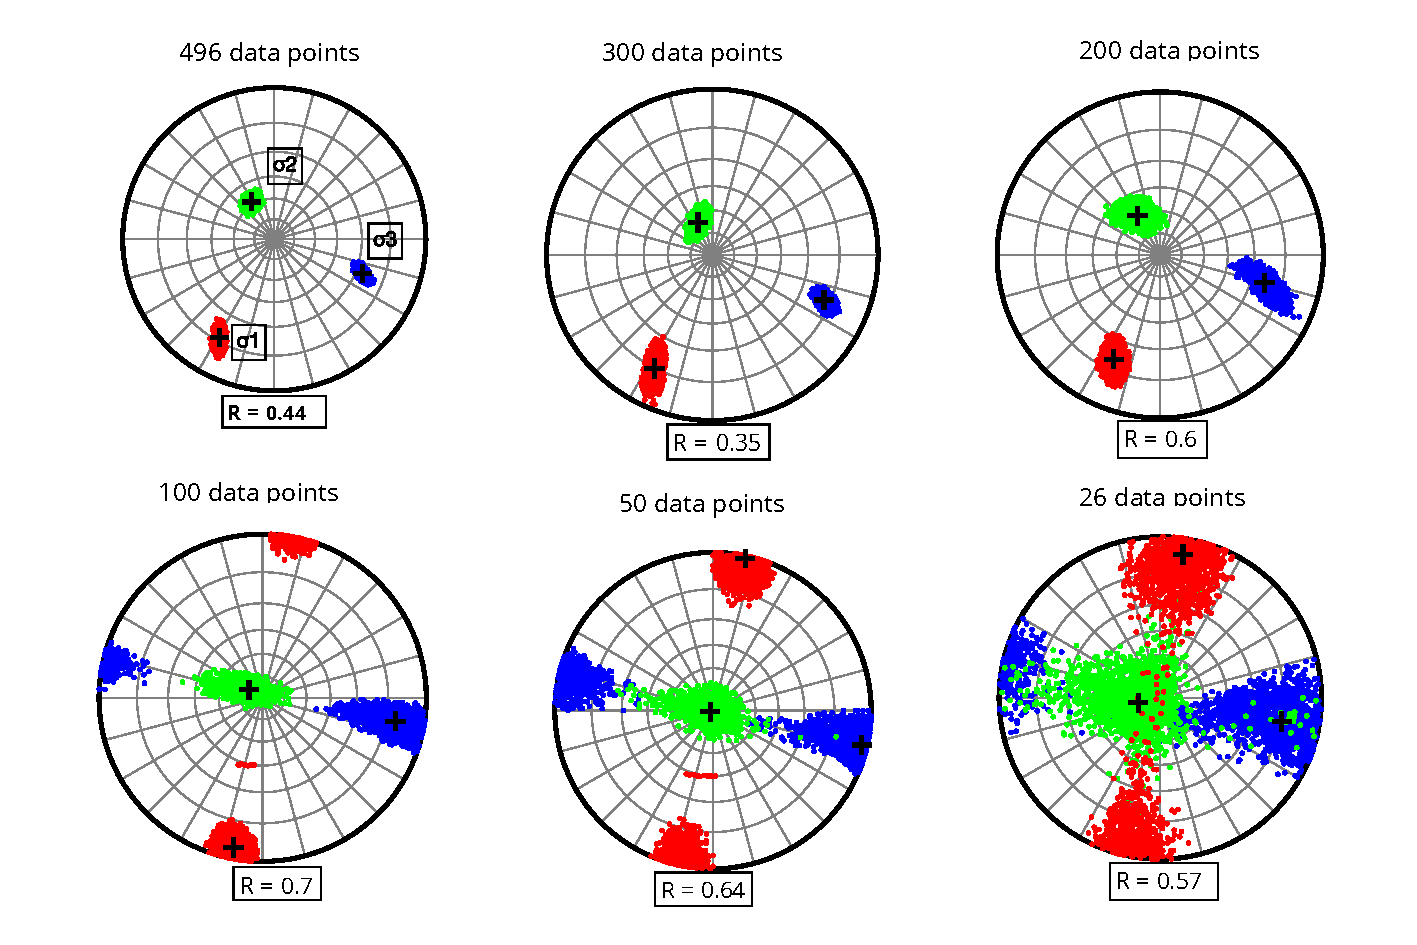
\includegraphics[scale=0.7]{data_uncert.pdf}
    \caption{Stress inversion for different number of data sets. We see that the first row of figures have similar principal stress orientations, but they become more uncertain as we reduce the number of data points. Another consideration is that though the principal stress orientation is better constrained for 200, 300, 496 data points, the stress ratio R is not.}
\end{figure}

The stress ratio is poorly constrained compared to the principal stress orientations because the inversion is highly nonlinear in terms of stress ratio and `msatsi' uses a linearized inversion scheme.

\section*{Uncertainty due to bootstrapping}
Here, we test the uncertainty due to number of bootstraps in our data set of 496 points. We successively  bootstrap 20, 200, 500, and 2000 times. We see that the best fit values of the stress ratio and the principal stress orientations do not change, but the uncertainty increases with increasing bootstraps. We also see that the uncertainty is not much different after increasing the bootstrapping from 200 times to 2000 times, therefore, for the given data set, it is enough to use a bootstrap resampling value of 200.


\begin{figure}[!htb]
    \centering
    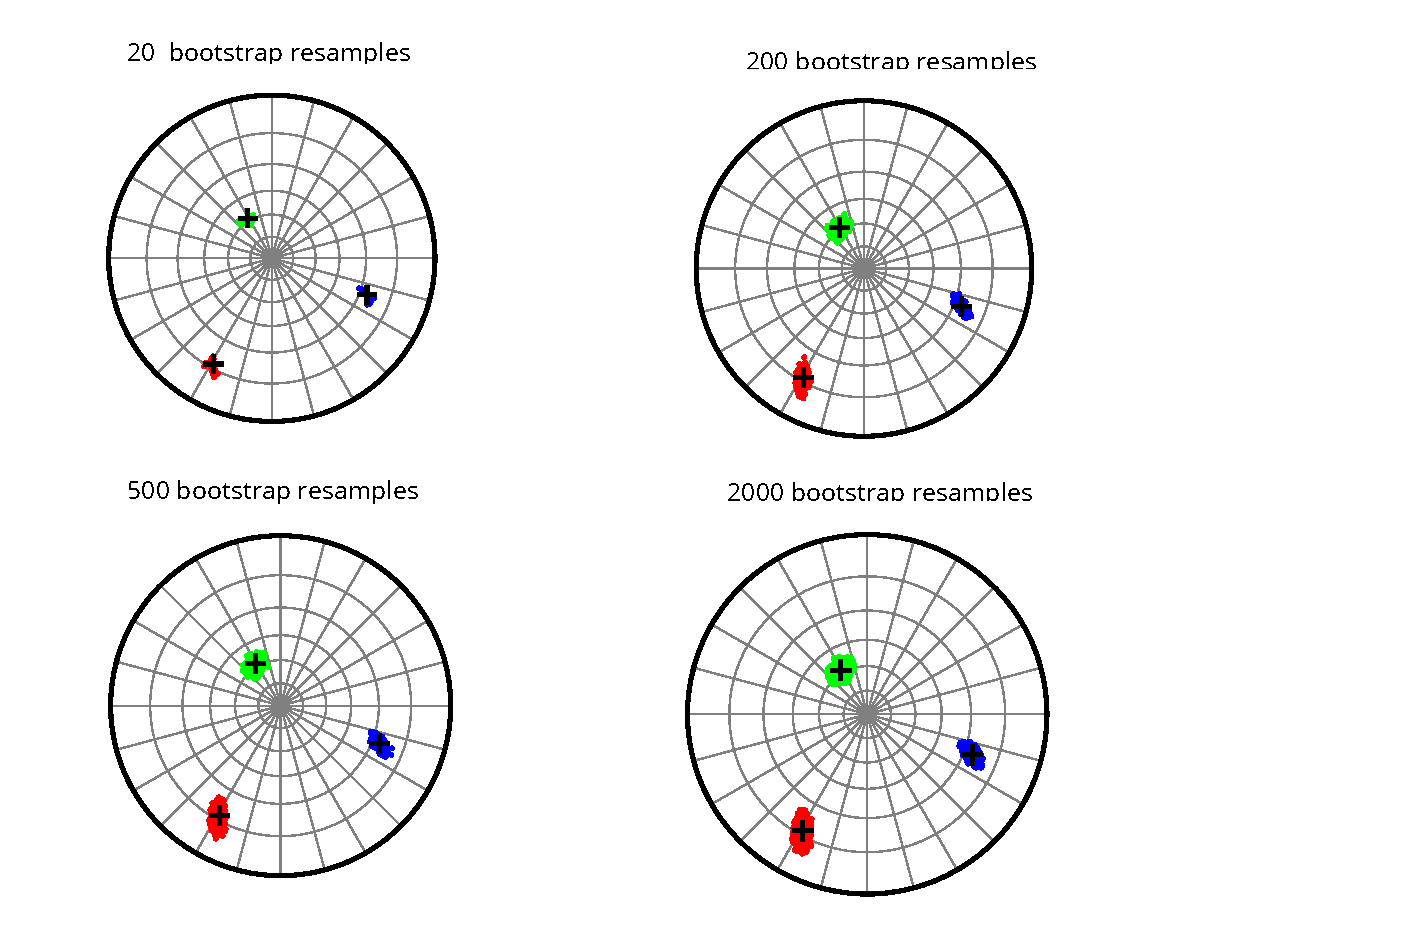
\includegraphics[scale=0.7]{bootstrap_uncert.pdf}
    \caption{Principal stress orientations for different bootstrap values. The stress ratio R = 0.44 in all the cases. The best-fit inversion values would be same but the number of bootstrap resamplings would provide with the uncertainties. We see that bootstrapping beyond 200 times doesn't change the uncertainties much.}
\end{figure}

\end{document}
